\section{Experiments}\label{sec:experiments}
We compute the constants of Sections~\ref{sec:general}--\ref{sec:population} exactly for trained models. Every population $P$ is a held-out or target empirical law mixed with a uniform mass of $1\%$ over profiles and labels, which gives full support; every design is pointwise unbiased; and every reported constant is certified by primal and dual bounds that agree to a relative error of at most $10^{-4}$. Ratios are $W_\A(P)/W_{\rm branch}(P)$, the factor by which the best design of a class needs more records than the best branching design. Protocols, every per-run value and sensitivity analyses are in Appendix~\ref{app:F}.

\paragraph{Forest updates.}
On WDBC, Spambase and Ionosphere \citep{wolberg1993,spambase1999,ionosphere1989}, an old and a new random forest of twenty depth-$b$ trees are trained on disjoint records with $m\in\{6,9,12\}$ median-binarized features, and the remaining 269, 3,101 and 171 records define $P$. The contrast is the difference of the forests' predicted probabilities, so no single tree computes it and even branching falls short of complete records. Table~\ref{tab:capgrid} reports caps two to four. At cap three the best pre-committed design needs a median \nCapThreeMed{} times as many records as the best branching design (range \nCapThreeMin--\nCapThreeMax), growing from \nCapThreeMsix{} at $m=6$ to \nCapThreeMtwelve{} at $m=12$. An exact optimal two-round design recovers \nTwoForestLo--\nTwoForestHi\% of the log-gap in each of the \nTwoForestN{} tasks where it was computed and needs at most \nTwoForestRatioMax{} times the records of branching. Branching restricted to the forests' own trees captures a median of only \nCapThreeShare\% of the log-gap at cap three: optimal branching designs mix many trees that neither forest contains. For these ensembles the cap costs more than pre-commitment does: relative to complete records, the best fixed designs need \nCapFixLo--\nCapFixHi{} and the best branching designs \nCapBrLo--\nCapBrHi{} times as many records (medians by cap).

\begin{table}[t]
\centering
\caption{Forest updates of depth $b$ under cap $b$ (WDBC, Spambase, Ionosphere; binding tasks). Fixed/branch: exact $W_{\rm fixed}/W_{\rm branch}$, median [minimum, maximum]. Fit: median excess of the ratio realized by designs optimized on training records over the exact ratio of the same task ($^\dagger$the 15 tasks with $m=12$). Own: share of the log-gap captured when branching may use only the forests\textquotesingle{} own trees. Two: exact optimal two-round design, $W_2/W_{\rm branch}$ ($^\ddagger$five splits per cell: 45 and 15 tasks; at $b=2$ two rounds are branching). Cap: $W_{\rm fixed}$ and $W_{\rm branch}$ relative to the full-information variance.}
\label{tab:capgrid}
\footnotesize
\setlength{\tabcolsep}{2.6pt}
\begin{tabular}{rrlrrrrr}
\toprule
 & & & & & & \multicolumn{2}{c}{Cap: /full} \\
$b$ & tasks & Fixed/branch & Fit & Own & Two & fixed & branch \\
\midrule
2 & 45 & 1.31 [1.12, 1.49] & +1\% & 49\% & 1 & 4.1 & 3.3 \\
3 & 180 & 1.51 [1.14, 1.85] & +2\%$^\dagger$ & 17\% & 1.04$^\ddagger$ & 3.5 & 2.3 \\
4 & 15 & 1.24 [1.13, 1.35] & +3\% & 26\% & 1.03$^\ddagger$ & 1.4 & 1.1 \\
\bottomrule
\end{tabular}
\end{table}

\begin{table*}[t]
\centering
\caption{Screening trees: records needed relative to branching, which asks the tree\textquotesingle s own questions and attains the full-information variance (medians over targets and seeds; the range is over runs). Best: optimal fixed design over all forms at the target law. Fitted: the same program on source records, evaluated at the target. Label: optimal fixed design whose form probabilities may depend on the label. Two: exact optimal two-round design (at $b=6$ the median includes certified upper bounds from feasible two-round designs for 4 runs, Table~\ref{tab:runs}). Two fit.: two-round design fitted on source records. Uniform: balanced random forms (uniform over all $\binom{12}b$ forms) with the optimal scores for that design. $1/\rho_P^2$, $N_P$: the ends of Theorem~\ref{thm:bracket}; PS: optimized path-set design. -- not computed.}
\label{tab:screening}
\footnotesize
\setlength{\tabcolsep}{5pt}
\begin{tabular}{lrrlrrrrrrrr}
\toprule
Data, $b$ & runs & Best & [min, max] & Fitted & Label & Two & Two fit. & Uniform & $1/\rho_P^2$ & PS & $N_P$ \\
\midrule
BRFSS, 3 & 6 & 1.00 & [1.00, 1.34] & 1.04 & 1.00 & 1.00 & 1.00 & 15.8 & 1.00 & 1.00 & 1.5 \\
BRFSS, 4 & 6 & 1.49 & [1.00, 1.75] & 1.57 & 1.48 & 1.00 & 1.01 & 21.7 & 1.18 & 1.53 & 3.3 \\
BRFSS, 5 & 6 & 1.35 & [1.18, 1.54] & 1.42 & 1.35 & 1.00 & 1.01 & 12.9 & 1.08 & 1.36 & 5.4 \\
BRFSS, 6 & 6 & 1.58 & [1.42, 1.98] & 1.68 & -- & $\le$1.05 & -- & 11.1 & 1.13 & 1.61 & 10.5 \\
Thyroid, 3--6 & 24 & 1.00 & [1.00, 1.00] & 1.04 & 1.00 & 1.00 & 1.04 & 4.9 & 1.00 & 1.00 & 3.6 \\
\addlinespace[2pt]
BRFSS-21, 3 & 3 & 1.00 & [1.00, 1.00] & 1.00 & -- & 1.00 & -- & -- & 1.00 & 1.00 & 1.5 \\
BRFSS-21, 4 & 3 & 1.46 & [1.41, 1.55] & 1.54 & -- & 1.00 & -- & -- & 1.18 & 1.50 & 3.5 \\
\bottomrule
\end{tabular}
\end{table*}


\paragraph{Screening questionnaires.}
A depth-$b$ screening tree asks at most $b$ questions per person, so a validation study under the same burden must respect the cap. We train class-balanced CART trees on twelve yes/no items of the CDC Diabetes Health Indicators, derived from the Behavioral Risk Factor Surveillance System (BRFSS; 253,680 respondents, target diabetes or prediabetes) \citep{cdcdiabetes2017}, and on twelve binarized thyroid items (7,200 patients, abnormal function) \citep{quinlan1986thyroid}, and validate them on a disjoint random half or on respondents of the other sex. Table~\ref{tab:screening} summarizes the runs and Table~\ref{tab:runs} lists each one.

\emph{The price of pre-commitment.} On BRFSS the best pre-committed design needs a median \nScreenBestLo--\nScreenBestHi{} times as many respondents at caps four to six (\nScreenRunLo--\nScreenRunHi{} over runs). On thyroid, and for the BRFSS trees that use at most $b$ items, one form explains the whole target ($\rho_P^2=1$) and pre-commitment costs nothing. Letting the form probabilities depend on the label, or on the label and sex, lowers the ratio by at most \nLabelMax\% and \nStratMax\%, so the cost is not an artifact of label-blind forms.

\emph{Design matters more than adaptivity.} Balanced random forms, the default of matrix sampling, need \nUnifLo--\nUnifHi{} times the records of branching at caps four to six even with the best scores for that design, and \nUnifHtLo--\nUnifHtHi{} times with plain inverse-probability scores. For a 95\% interval of $\pm2$ accuracy points at $b=5$, branching needs about \nSsBranch{} respondents, optimized forms \nSsFixed{} and balanced random forms \nSsUnif{} (medians). The optimized designs concentrate on a few forms: restricting them to the tree's own path sets loses a median \nPsGapMed\% (at most \nPsGapMax\%) over the \nPsGapN{} runs with a gain, which also makes the upper end of the bracket tight, whereas the lower end $1/\rho_P^2$ is below the realized ratio by a median factor \nLowUnder{} and completion-only path guessing ($N_P$) is above it by \nNpOver.

\emph{One adaptive round.} \nCompBrfss{} of the \nBrfssRuns{} BRFSS trees, and the three 21-item trees, are computed exactly by a two-round interview with at most $b$ questions, so for them a second round removes the whole cost. For the other trees the exact optimal two-round design needs at most \nScreenTwoMax{} times the records of branching in the \nScreenTwoN{} runs with a gain that were solved to optimality (every run at $b\le5$ and \nSixExact{} at $b=6$). For the remaining \nTwoBounded{} runs at $b=6$ column generation was stopped after one hour; the feasible two-round designs found by then need between \nTwoBoundMin{} and \nTwoBoundMax{} times the records of branching, so the second round recovers at least \nTwoBoundRec\% of the log-gap there. A two-round design fitted on source records needs a median \nScreenTwoFitMed{} (at most \nScreenTwoFitMax) at $b\le5$. The heuristic of following the root question and then the best fixed form recovers only \nHeurLo--\nHeurHi\%. With the forest results, a second round recovered at least \nTwoMinPct\% of the log-gap in every case solved to optimality, far from the worst case of Theorem~\ref{thm:rounds}.

\begin{figure}[t]
\centering
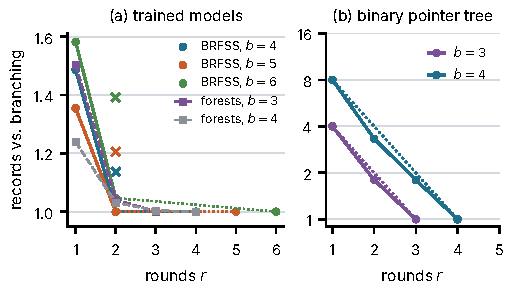
\includegraphics[width=\columnwidth]{figures/v15_rounds.pdf}
\caption{Records needed relative to branching as a function of the number of rounds ($r=1$: fixed forms; $r=b$: branching). (a) Optimal $r$-round designs for BRFSS screening trees (median over targets and seeds; at $b=6$ and $r=2$ the median includes upper bounds) and forest updates (median over tasks); crosses mark the heuristic second round of following the root question. (b) Binary pointer tree under the uniform law, a lower bound on $V_r$ (Appendix~\ref{app:pointerexact}); dotted lines are the upper bounds $2^{b-r}$ of Theorem~\ref{thm:rounds}(a).}
\label{fig:rounds}
\end{figure}

\paragraph{Deployable designs.}
Fixed designs fitted on 20,000 source records need a median \nFitMed\% (at most \nFitMax\%) more records than the oracle designs and remain exactly unbiased. Without a reference, the design can be learned from a pilot of the audit itself (Proposition~\ref{prop:selfcalmain}): with a pilot of 1,000 respondents on the tree's path sets, the learned design needs a median \nPilotFourNc\% more records than the oracle path-set design at $b=4$ (\nPilotFourCells{} cell masses to estimate) and \nPilotFiveNc\% at $b=5$ (\nPilotFiveCells{} cells); with 4,000 respondents the excess is \nPilotFourNe\%, \nPilotFiveNe\% and \nPilotSixNe\% at $b=4,5,6$ (Table~\ref{tab:pilot}). Learning needs a pilot of several times the number of cell masses, so at larger caps a reference is worth having.

\paragraph{All 21 survey variables.}
With all 21 BRFSS variables the cube has $2^{21}$ profiles and the form program has 5,985 forms at $b=4$; the solver certifies the optimal fixed design against all of them, without enumerating the cube, in a median of \nScaleMin{} minutes on one core. The trees select the same items as in the twelve-item study, so the constants are those of runs R0--R2; the study tests the size of the program, not a new population (Appendix~\ref{app:scale}).

\paragraph{Design-based versus model-based estimation.}
\nModelParagraph

\paragraph{Order effects.}
If the last of $b$ answers flips with probability $0.1$ and earlier ones proportionally less often, both designs are biased: on BRFSS the median absolute bias at $n=1000$ is \nPosBranch{} clean branching standard errors for branching and \nPosFit{} for the fitted fixed form, comparable to the sampling gains above, and branching keeps the smaller RMSE in \nPosWin{} of \nPosN{} runs (Appendix~\ref{app:measurement}). This is an illustrative response model, not an estimated one.
